\section{Einleitung}

Im Rahmen des Klimarisiko-Stresstests 2022 konzentrierte sich die Bewertung physischer Risiken auf zwei extreme Wetterereignisse, die zentrale Klimarisiken in Europa darstellen: (1) eine große Überschwemmung und (2) eine schwere Dürre mit Hitzewelle \parencite{ECB2022ClimateStressTest}. Flussüberschwemmungen waren historisch betrachtet eine bedeutende Quelle physischer Risiken in Europa und werden aufgrund prognostizierter Niederschlagszunahmen voraussichtlich an Relevanz gewinnen.
Diese Arbeit fokussiert sich spezifisch auf das Flusshochwasserrisiko in Bayern, Deutschland. Diese Eingrenzung ermöglicht eine detaillierte Analyse der regionalen Auswirkungen und Anpassungsstrategien im Kontext physischer Klimarisiken für den bayerischen Immobiliensektor.

Im Folgenden wird beispielhaft gezeigt, wie Zitate, Bilder, Tabellen oder Quellcode in die Arbeit eingefügt werden können.

\subsection{Zitate}
Menschen, die mit ihrem IQ prahlen, sind Versager.

\subsection{Bilder}
\begin{figure}[H] 
    \centering
    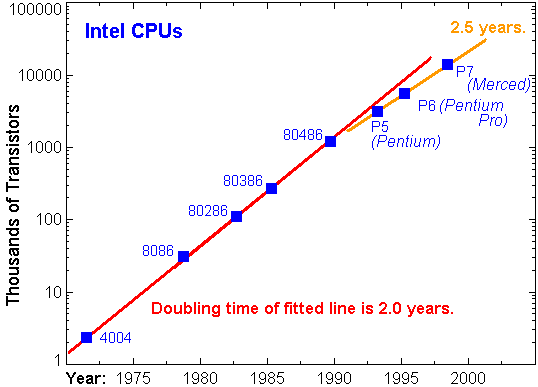
\includegraphics[width=0.5\textwidth]{figures/figure_example.png}
    \caption{Mooresches Gesetz}
\end{figure}

\subsection{Tabellen}
\begin{table}[H]
    \centering
    \begin{tabular}[H]{l|l|l}
        Bezeichnung & Kerne & TDP \\
        \hline
        Intel Core i5 & 6 & 111 W \\
        \hline
        AMD Ryzen 7 & 8 & 178 W \\
    \end{tabular}
    \caption{Prozessoren}
\end{table}


\subsection{Quellcode}
\begin{lstlisting}[language=java, caption=Hello World in Java, captionpos=b]
    class HelloWorld {
        public static void main(String[] args) {
            // Display the string.y
            System.out.println("Hello World!");
        }
    }
\end{lstlisting}
